% A nonlinear vertical rescaling: this grid does NOT represent the same line bundle structure.
% Source: book/tex/riemann-surface/line-bundles.tex (asy figure).
\documentclass[border=2mm]{standalone}
\usepackage{tikz}
\begin{document}
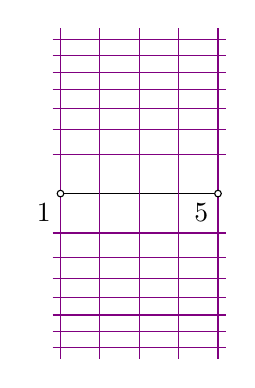
\begin{tikzpicture}[scale=0.5,>=latex]
  \draw (1,0) -- (5,0);
  \node[anchor=north east] at (1,0) {$1$};
  \node[anchor=north east] at (5,0) {$5$};
  \draw[violet] (1,-4.2) -- (1,4.2);
  \draw[violet] (2,-4.2) -- (2,4.2);
  \draw[violet] (3,-4.2) -- (3,4.2);
  \draw[violet] (4,-4.2) -- (4,4.2);
  \draw[violet] (5,-4.2) -- (5,4.2);
  \draw[violet] (0.8,-3.9045) -- (5.2,-3.9045);
  \draw[violet] (0.8,-3.5051) -- (5.2,-3.5051);
  \draw[violet] (0.8,-3.0852) -- (5.2,-3.0852);
  \draw[violet] (0.8,-2.6390) -- (5.2,-2.6390);
  \draw[violet] (0.8,-2.1577) -- (5.2,-2.1577);
  \draw[violet] (0.8,-1.6245) -- (5.2,-1.6245);
  \draw[violet] (0.8,-1.0000) -- (5.2,-1.0000);
  \draw[violet] (0.8,1.0000) -- (5.2,1.0000);
  \draw[violet] (0.8,1.6245) -- (5.2,1.6245);
  \draw[violet] (0.8,2.1577) -- (5.2,2.1577);
  \draw[violet] (0.8,2.6390) -- (5.2,2.6390);
  \draw[violet] (0.8,3.0852) -- (5.2,3.0852);
  \draw[violet] (0.8,3.5051) -- (5.2,3.5051);
  \draw[violet] (0.8,3.9045) -- (5.2,3.9045);
  \filldraw[fill=white] (1,0) circle (2.4pt);
  \filldraw[fill=white] (5,0) circle (2.4pt);
\end{tikzpicture}
\end{document}
